\documentclass[12pt,fleqn]{article}\usepackage{../../common}
\begin{document}
Da�lar Aras�nda En Optimal Y�r�y�� Yolu Bulmak

\begin{minted}[fontsize=\footnotesize]{python}
from mpl_toolkits.mplot3d import Axes3D
from scipy.spatial.distance import cdist
from matplotlib import cm

def gfunc(x, y):
    s1 = 2.2; x1 = 2.0; y1 = 2.0
    g1 = np.exp( -4 *np.log(2) * ((x-x1)**2+(y-y1)**2) / s1**2)
    return g1 

def plot_surf_path(a0,a1,a2,a3,a4,b0,b1,b2,b3,b4):

    D = 50
    x = np.linspace(0,5,D)
    y = np.linspace(0,5,D)
    xx,yy = np.meshgrid(x,y)
    zz = gfunc(xx,yy)

    fig = plt.figure()
    ax = fig.gca(projection='3d')
    ax.set_xlim(0,5)
    ax.set_ylim(0,5)
    surf = ax.plot_wireframe(xx, yy, zz,rstride=10, cstride=10)

    t = np.linspace(0,1.0,100)

    x = a0 + a1*t + a2*t**2 + a3*t**3 + a4*t**4 
    y = b0 + b1*t + b2*t**2 + b3*t**3 + b4*t**4

    ax.plot3D(x, y, gfunc(x,y),'r.')

# 1. gidis yolunun tanimi, uzun yoldan dolanarak gidiyor
a1,a2,a3 = 1.5, 8.1, 4.0
b1,b2,b3 = 0.3, 0.4, 23.3
a0,b0=(1.0,1.0)
ex,ey=(0.3,4.0)
a4 = ex - a0 - (a1+a2+a3)
b4 = ey - b0 - (b1+b2+b3)
test_coefs1 = (a0,a1,a2,a3,a4,b0,b1,b2,b3,b4)
plot_surf_path(a0,a1,a2,a3,a4,b0,b1,b2,b3,b4)

plt.savefig('calc_multi_40_elev_01.png')
\end{minted}

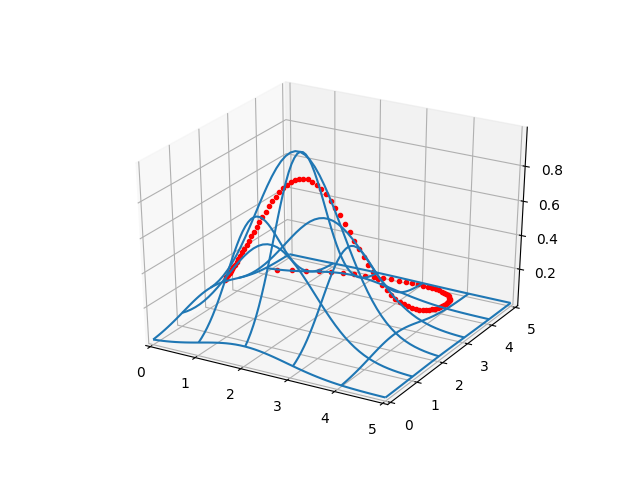
\includegraphics[width=20em]{calc_multi_40_elev_01.png}

\begin{minted}[fontsize=\footnotesize]{python}
t = np.linspace(0,1.0,100)
x = a0 + a1*t + a2*t**2 + a3*t**3 + a4*t**4 
y = b0 + b1*t + b2*t**2 + b3*t**3 + b4*t**4
plt.xlim(0,5.0)
plt.ylim(0,5.0)
plt.plot(x,y)
plt.savefig('calc_multi_40_elev_02.png')
\end{minted}

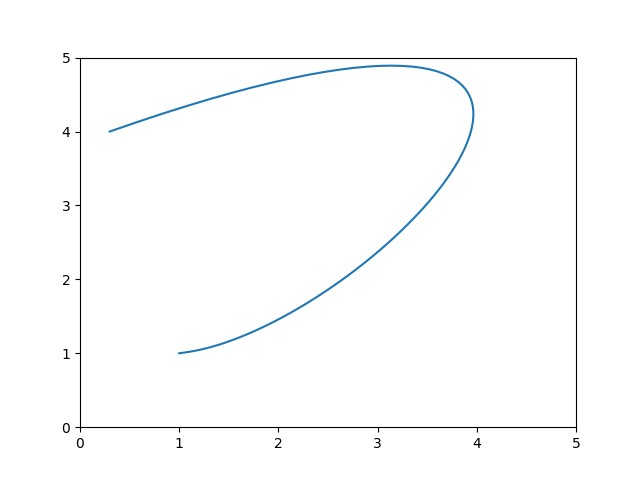
\includegraphics[width=20em]{calc_multi_40_elev_02.png}

\begin{minted}[fontsize=\footnotesize]{python}
# 2. gidis yolunun tanimi, dik cikip iniyor
a1,a2,a3 = 1.5, 3.0, 1.0
b1,b2,b3 = 0.0, 1.0, 1.0
a0,b0=(1.0,1.0)
ex,ey=(0.3,4.0)
a4 = ex - a0 - (a1+a2+a3)
b4 = ey - b0 - (b1+b2+b3)
test_coefs2 = (a0,a1,a2,a3,a4,b0,b1,b2,b3,b4)
plot_surf_path(a0,a1,a2,a3,a4,b0,b1,b2,b3,b4)
plt.savefig('calc_multi_40_elev_03.png')
\end{minted}

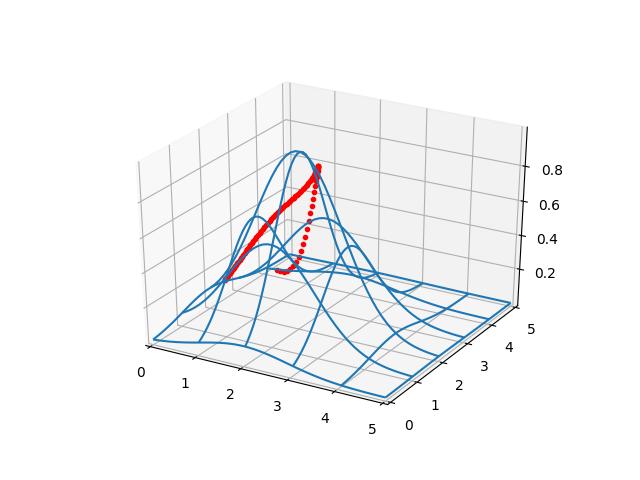
\includegraphics[width=20em]{calc_multi_40_elev_03.png}

$$
\int_{t=0}^{t=1} f(x(t),y(t)) \sqrt{(\ud x/\ud t)^2 + (\ud y/\ud t)^2} \ud t
$$

\begin{minted}[fontsize=\footnotesize]{python}
import sympy

vars = 't a0 a1 a2 a3 b0 b1 b2 b3 gamma x y'
t, a0, a1, a2, a3, b0, b1, b2, b3, gamma, x, y = sympy.symbols(vars)

xdef = a0 + a1*t + a2*t**2 + a3*t**3 + a4*t**4
ydef = b0 + b1*t + b2*t**2 + b3*t**3 + b4*t**4

dxdt = sympy.diff(xdef,t)
print (dxdt)
dydt = sympy.diff(ydef,t)
print (dydt)
sqrtdef = sympy.sqrt(sympy.diff(xdef,t)**2 + sympy.diff(ydef,t))
print (sqrtdef)
\end{minted}

\begin{verbatim}
a1 + 2*a2*t + 3*a3*t**2 - 57.2*t**3
b1 + 2*b2*t + 3*b3*t**2 - 84.0*t**3
sqrt(b1 + 2*b2*t + 3*b3*t**2 - 84.0*t**3 + (a1 + 2*a2*t + 3*a3*t**2 - 57.2*t**3)**2)
\end{verbatim}


\begin{minted}[fontsize=\footnotesize]{python}
def trapz(y, dx):
    vals = np.nan_to_num(y[1:-1],0)
    tmp = np.sum(vals*2.0)    
    return (y[0]+tmp+y[-1])*(dx/2.0)

def intval(t,a0,a1,a2,a3,a4,b0,b1,b2,b3,b4):
   sq = np.sqrt(b1 + 2*b2*t + 3*b3*t**2 - 112.0*t**3 + (a1 + 2*a2*t + 3*a3*t**2 - 65.2*t**3)**2)
   x = a0 + a1*t + a2*t**2 + a3*t**3 + a4*t**4 
   y = b0 + b1*t + b2*t**2 + b3*t**3 + b4*t**4
   x = np.array(x)
   y = np.array(y)   
   z = gfunc(x,y)   
   res = z * sq
   T = trapz(res, 1.0/len(t))
   return T

t = np.linspace(0,1,100)

a0,a1,a2,a3,a4,b0,b1,b2,b3,b4 = test_coefs1
T = intval(t,a0,a1,a2,a3,a4,b0,b1,b2,b3,b4)
print (T)
a0,a1,a2,a3,a4,b0,b1,b2,b3,b4 = test_coefs2
T = intval(t,a0,a1,a2,a3,a4,b0,b1,b2,b3,b4)
print (T)
\end{minted}

\begin{verbatim}
1.624956808796678
5.534245013919315
\end{verbatim}




\begin{minted}[fontsize=\footnotesize]{python}
(a1,a2,a3,b1,b2,b3) = (-3.99250585,  0.40668743,  2.40068662,  8.67203816,  5.37002513, 2.82998489)
a0,b0=1.0,1.0
a0,b0=(1.0,1.0)
ex,ey=(0.3,4.0)
a4 = ex - a0 - (a1+a2+a3)
b4 = ey - b0 - (b1+b2+b3)
plot_surf_path(a0,a1,a2,a3,a4,b0,b1,b2,b3,b4)
plt.savefig('/tmp/out1.png')
\end{minted}










[devam edecek]

Kaynaklar 

[1] Bayraml�, Say�sal Bilim, {\em Say�sal Entegrasyon (Numerical Integration)}

[2] Bayraml�, Cok Boyutlu Calculus, {\em Ders 19, Skalar Alanlar Uzerinden Cizgi Entegral}

[2] Bayraml�, Cok Boyutlu Calculus, {\em Ders 5, �ki Nokta Aras�nda Parametrize Edilmi� E�ri}

\end{document}
